
\let\negmedspace\undefined
\let\negthickspace\undefined
\documentclass[journal,12pt,onecolumn]{IEEEtran}
\usepackage{cite}
\usepackage{amsmath,amssymb,amsfonts,amsthm}
\usepackage{algorithmic}
\usepackage{amsmath}
\usepackage{graphicx}
\graphicspath{{./figs/}}
\usepackage{textcomp}
\usepackage{framed} 

\usepackage[utf8]{inputenc}
\usepackage{xcolor}
\usepackage{txfonts}
\usepackage{romannum}
\usepackage{listings}
\usepackage{enumitem}
\usepackage{mathtools}
\usepackage{gensymb}
\usepackage{comment}
\usepackage{caption}
\usepackage[breaklinks=true]{hyperref}
\usepackage{tkz-euclide} 
\usepackage{listings}
\usepackage{gvv}                                        
\usepackage{color}        
\usepackage[utf8]{inputenc}                                     
\usepackage{array}                                            
\usepackage{longtable}         
\usepackage{multicol}                              
\usepackage{calc}                                             
\usepackage{multirow}
\usepackage{multicol}
\usepackage{hhline}                                           
\usepackage{ifthen}                                           
\usepackage{lscape}
\usepackage{tabularx}
\usepackage{array}
\usepackage{float}
\newtheorem{theorem}{Theorem}[section]
\newtheorem{problem}{Problem}
\newtheorem{proposition}{Proposition}[section]
\newtheorem{lemma}{Lemma}[section]
\newtheorem{corollary}[theorem]{Corollary}
\newtheorem{example}{Example}[section]
\newtheorem{definition}[problem]{Definition}
\newcommand{\BEQA}{\begin{eqnarray}}
	\newcommand{\EEQA}{\end{eqnarray}}

\theoremstyle{remark}


\title{\textbf{GATE CS 2020}}
\author{ EE25BTECH11052 - Shriyansh Kalpesh Chawda}
\begin{document}
	
	\maketitle
	{\huge GA - General Aptitude}\\
	\\
	\fbox{{\large Q.1 - Q.5 Carry ONE mark each}}\\
	\\
	\begin{enumerate}
		\item Raman is confident of speaking English \underline{\hspace{2cm}} six months as he has been practising regularly \underline{\hspace{2cm}} the last three weeks.
		
		\hfill{\brak{\text{GATE CS 2020}}}
		\begin{enumerate}
			\begin{multicols}{4}
				\item during, for
				\item for, since
				\item for, in
				\item within, for
			\end{multicols}
		\end{enumerate}
		
		\item His knowledge of the subject was excellent but his classroom performance was\underline{\hspace{2cm}}.
		
		\hfill{\brak{\text{GATE CS 2020}}}
		\begin{enumerate}
			\begin{multicols}{4}
				\item extremely poor
				\item good
				\item desirable
				\item praiseworthy
			\end{multicols}
		\end{enumerate}
		
		\item Select the word that fits the analogy:
		Cook $\colon$ Cook $\colon\colon$ Fly $\colon$ \underline{\hspace{2cm}}
		
		\hfill{\brak{\text{GATE CS 2020}}}
		\begin{enumerate}
			\begin{multicols}{4}
				\item Flyer
				\item Flying
				\item Flew
				\item Flighter
			\end{multicols}
		\end{enumerate}
		
		\item The dawn of the 21st century witnessed the melting glaciers oscillating between giving too much and too little to billions of people who depend on them for fresh water. The UN climate report estimates that without deep cuts to man-made emissions, at least $30\%$ of the northern hemisphere’s surface permafrost could melt by the end of the century. Given this situation of imminent global exodus of billions of people displaced by rising seas, nation-states need to rethink their carbon footprint for political concerns, if not for environmental ones.
		Which one of the following statements can be inferred from the given passage?
		
		\hfill{\brak{\text{GATE CS 2020}}}
		\begin{enumerate}
			\item Nation-states do not have environmental concerns.
			\item Nation-states are responsible for providing fresh water to billions of people.
			\item Billions of people are responsible for man-made emissions.
			\item Billions of people are affected by melting glaciers.
		\end{enumerate}
		
		\item There are multiple routes to reach from node $1$ to node $2$, as shown in the network.
	
		The cost of travel on an edge between two nodes is given in rupees. Nodes `a', `b', `c', `d', `e', and `f' are toll booths. The toll price at toll booths marked `a' and `e' is Rs. $200$, and is Rs. $100$ for the other toll booths. Which is the cheapest route from node $1$ to node $2$?
		\begin{figure}[H]
			\centering
			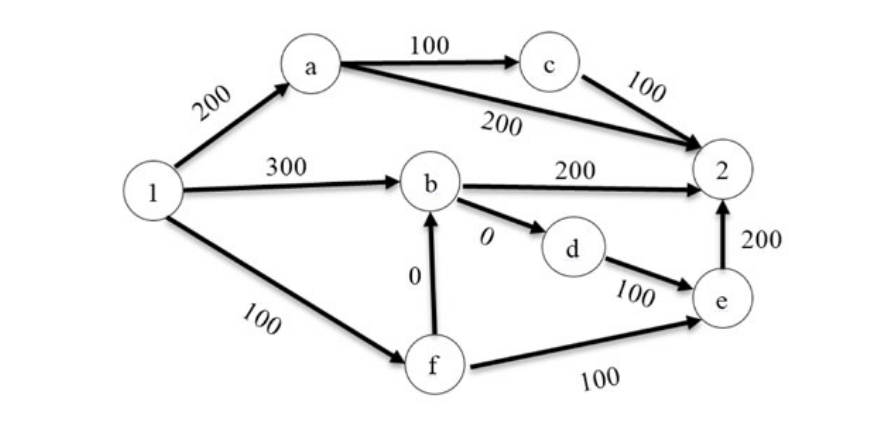
\includegraphics[width=0.6\linewidth]{figs/1}
			\caption{}
			\label{fig:1}
		\end{figure}
		
		\hfill{\brak{\text{GATE CS 2020}}}
		\begin{enumerate}
			\begin{multicols}{2}
				\item 1-a-c-2
				\item 1-f-b-2
				\item 1-b-2
				\item 1-f-e-2
			\end{multicols}
		\end{enumerate}
		\fbox{{\Large Q.6 - Q.10 Carry ONE mark each}}
		\vspace{1cm}
		\item Goods and Services Tax \brak{\text{GST}} is an indirect tax introduced in India in $2017$ that is imposed on the supply of goods and services, and it subsumes all indirect taxes except few. It is a destination-based tax imposed on goods and services used, and it is not imposed at the point of origin from where goods come. GST also has a few components specific to state governments, central government and Union Territories \brak{\text{UTs}}.
		Which one of the following statements can be inferred from the given passage?
		
		\hfill{\brak{\text{GATE CS 2020}}}
		\begin{enumerate}
			\item GST is imposed on the production of goods and services.
			\item GST includes all indirect taxes.
			\item GST does not have a component specific to UT.
			\item GST is imposed at the point of usage of goods and services.
		\end{enumerate}
		

		

		\item If $P=3, R=27, T=243, \text{ then } Q+S = $ \underline{\hspace{2cm}}.
		
		\hfill{\brak{\text{GATE CS 2020}}}
		\begin{enumerate}
			\begin{multicols}{4}
				\item $40$
				\item $80$
				\item $90$
				\item $110$
			\end{multicols}
		\end{enumerate}
		
		\item The figure below shows an annular ring with outer and inner radii as $b$ and $a$, respectively. The annular space has been painted in the form of blue colour circles touching the outer and inner periphery of annular space. If maximum $n$ number of circles can be painted, then the unpainted area available in annular space is \underline{\hspace{2cm}}.
		\begin{figure}[H]
			\centering
			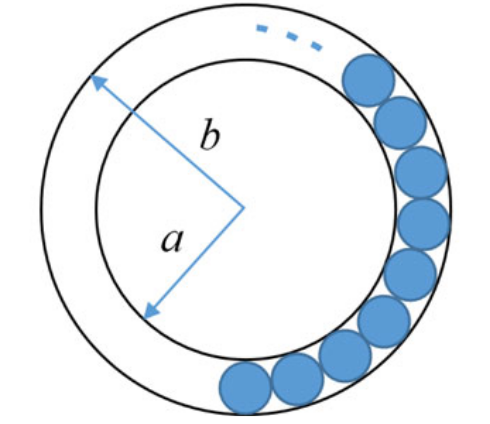
\includegraphics[width=0.45\linewidth]{figs/2}
			\caption{}
			\label{fig:2}
		\end{figure}
		
		
		\hfill{\brak{\text{GATE CS 2020}}}
		\begin{enumerate}
			\item $\pi \left[ \brak{b^2-a^2} - \frac{n}{4}\brak{b-a}^2 \right]$
			\item $\pi \left[ \brak{b^2-a^2} - n\brak{b-a}^2 \right]$
			\item $\pi \left[ \brak{b^2-a^2} + \frac{n}{4}\brak{b-a}^2 \right]$
			\item $\pi \left[ \brak{b^2-a^2} + n\brak{b-a}^2 \right]$
		\end{enumerate}
		
		\item Two straight lines are drawn perpendicular to each other in X-Y plane. If $\alpha$ and $\beta$ are the acute angles the straight lines make with the X-axis, then $\alpha + \beta$ is \underline{\hspace{2cm}}.
		
		\hfill{\brak{\text{GATE CS 2020}}}
		\begin{enumerate}
			\begin{multicols}{4}
				\item $60\degree$
				\item $90\degree$
				\item $120\degree$
				\item $180\degree$
			\end{multicols}
		\end{enumerate}
		
		\item The total revenue of a company during 2014-2018 is shown in the bar graph. If the total expenditure of the company in each year is 500 million rupees, then the aggregate profit or loss \brak{\text{in percentage}} on the total expenditure of the company during 2014-2018 is \underline{\hspace{2cm}}.
		\begin{figure}[H]
			\centering
			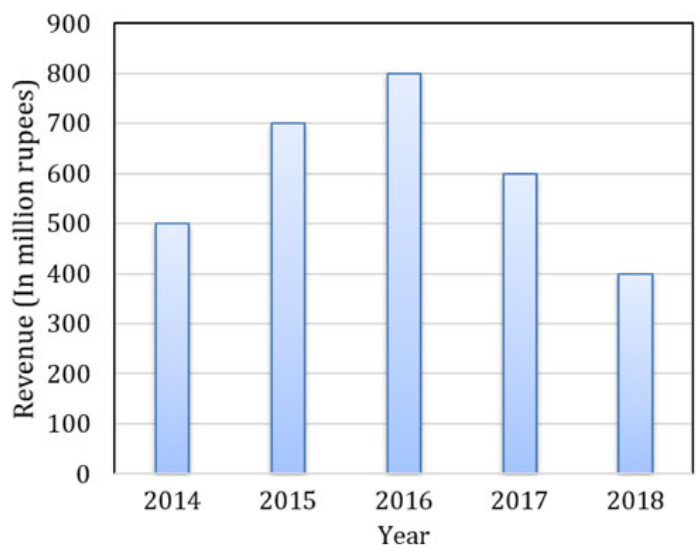
\includegraphics[width=0.6\linewidth]{figs/3}
			\caption{}
			\label{fig:3}
		\end{figure}
		
		
		\hfill{\brak{\text{GATE CS 2020}}}
		\begin{enumerate}
			\begin{multicols}{2}
				\item $16.67$ \% profit
				\item $16.67$ \% loss
				\item $20$ \% profit
				\item $20$ \% loss
			\end{multicols}
		\end{enumerate}
\end{enumerate}
\pagebreak

\fbox{{\Large Q.1 - Q.25 Carry ONE mark each}}\\
\\

\begin{enumerate}
	\item Consider the functions
	\begin{enumerate}
		\item[I.] $e^{-x}$
		\item[II.] $x^2 - \sin x$
		\item[III.] $\sqrt{x^3 + 1}$
	\end{enumerate}
	Which of the above functions is/are increasing everywhere in $[0,1]$?
	
	\hfill{\brak{\text{GATE CS 2020}}}
	\begin{enumerate}
		\begin{multicols}{4}
			\item III only
			\item II only
			\item II and III only
			\item I and III only
		\end{multicols}
	\end{enumerate}
	
	\item For parameters $a$ and $b$, both of which are $\omega\brak{1}$, $T\brak{n} = T\brak{n^{1/a}} + 1$, and $T\brak{b}=1$.
	Then $T\brak{n}$ is
	
	\hfill{\brak{\text{GATE CS 2020}}}
	\begin{enumerate}
		\begin{multicols}{4}
			\item $\Theta\brak{\log_a \log_b n}$
			\item $\Theta\brak{\log_{ab} n}$
			\item $\Theta\brak{\log_b \log_a n}$
			\item $\Theta\brak{\log_2 \log_2 n}$
		\end{multicols}
	\end{enumerate}
	
	\item Consider the following statements.
	\begin{enumerate}
		\item[I.] Daisy chaining is used to assign priorities in attending interrupts.
		\item[II.] When a device raises a vectored interrupt, the CPU does polling to identify the source of interrupt.
		\item[III.] In polling, the CPU periodically checks the status bits to know if any device needs its attention.
		\item[IV.] During DMA, both the CPU and DMA controller can be bus masters at the same time.
	\end{enumerate}
	Which of the above statements is/are TRUE?
	\hfill{\brak{\text{GATE CS 2020}}}
	\begin{enumerate}
		\begin{multicols}{4}
			\item I and II only
			\item I and IV only
			\item I and III only
			\item III only
		\end{multicols}
	\end{enumerate}
	
	\item Consider the following data path diagram.
	
	Consider an instruction: R0 $\leftarrow$ R1 + R2. The following steps are used to execute it over the given data path. Assume that PC is incremented appropriately. The subscripts r and w indicate read and write operations, respectively.Consider the following data path diagram.
	\begin{figure}[H]
		\centering
		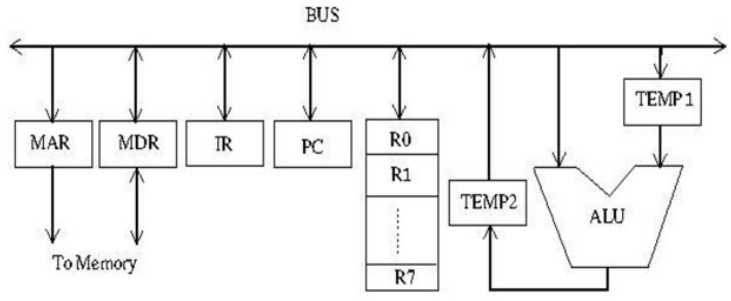
\includegraphics[width=0.5\linewidth]{figs/4}
		\caption{}
		\label{fig:4}
	\end{figure}
	
	\begin{enumerate}
		\item R2$_r$, TEMP1$_w$, ALU$_{add}$, TEMP2$_w$
		\item R1$_r$, TEMP1$_w$
		\item PC$_r$, MAR$_w$, MEM$_r$
		\item TEMP2$_r$, R0$_w$
		\item MDR$_r$, IR$_w$
	\end{enumerate}
	Which one of the following is the correct order of execution of the above steps?
	
	\hfill{\brak{\text{GATE CS 2020}}}
	\begin{enumerate}
		\begin{multicols}{2}
			\item 2, 1, 4, 5, 3
			\item 1, 2, 4, 3, 5
			\item 3, 5, 2, 1, 4
			\item 3, 5, 1, 2, 4
		\end{multicols}
	\end{enumerate}
	
	\item The preorder traversal of a binary search tree is 15, 10, 12, 11, 20, 18, 16, 19.
	Which one of the following is the postorder traversal of the tree?
	
	\hfill{\brak{\text{GATE CS 2020}}}
	\begin{enumerate}
		\item 10, 11, 12, 16, 18, 19, 20
		\item 11, 12, 10, 16, 19, 18, 20, 15
		\item 20, 19, 18, 16, 15, 12, 11, 10
		\item 19, 16, 18, 20, 11, 12, 10, 15
	\end{enumerate}
	
	\item What is the worst case time complexity of inserting $n^2$ elements into an AVL-tree with $n$ elements initially?
	
	\hfill{\brak{\text{GATE CS 2020}}}
	\begin{enumerate}
		\begin{multicols}{4}
			\item $\Theta\brak{n^4}$
			\item $\Theta\brak{n^2}$
			\item $\Theta\brak{n^2 \log n}$
			\item $\Theta\brak{n^3}$
		\end{multicols}
	\end{enumerate}
	
	\item Which one of the following regular expressions represents the set of all binary strings with an odd number of 1’s?
	
	\hfill{\brak{\text{GATE CS 2020}}}
	\begin{enumerate}
		\item $\brak{\brak{0+1}^*1\brak{0+1}^*1}^*10^*$
		\item $\brak{0^*10^*10^*}^*0^*10^*$
		\item $10^*\brak{0^*10^*10^*}^*$
		\item $\brak{0^*10^*10^*}^*10^*$
	\end{enumerate}
	
	\item Consider the following statements.
	\begin{enumerate}
		\item[I.] If $L_1 \cup L_2$ is regular, then both $L_1$ and $L_2$ must be regular.
		\item[II.] The class of regular languages is closed under infinite union.
	\end{enumerate}
	Which of the above statements is/are TRUE?
	\hfill{\brak{\text{GATE CS 2020}}}
	\begin{enumerate}
		\begin{multicols}{4}
			\item I only
			\item II only
			\item Both I and II
			\item Neither I nor II
		\end{multicols}
	\end{enumerate}
	
	\item Consider the following statements.
	\begin{enumerate}
		\item[I.] Symbol table is accessed only during lexical analysis and syntax analysis.
		\item[II.] Compilers for programming languages that support recursion necessarily need heap storage for memory allocation in the run-time environment.
		\item[III.] Errors violating the condition ‘\textit{any variable must be declared before its use}’ are detected during syntax analysis.
	\end{enumerate}
	Which of the above statements is/are TRUE?
	\hfill{\brak{\text{GATE CS 2020}}}
	\begin{enumerate}
		\begin{multicols}{4}
			\item I only
			\item I and III only
			\item II only
			\item None of I, II, and III
		\end{multicols}
	\end{enumerate}
	
	\item Consider the language $L = \{a^n \mid n \ge 0\} \cup \{a^n b^n \mid n \ge 0\}$ and the following statements.
	\begin{enumerate}
		\item[I.] $L$ is deterministic context-free.
		\item[II.] $L$ is context-free but not deterministic context-free.
		\item[III.] $L$ is not LL$\brak{k}$ for any $k$.
	\end{enumerate}
	Which of the above statements is/are TRUE?
	
	\hfill{\brak{\text{GATE CS 2020}}}
	\begin{enumerate}
		\begin{multicols}{4}
			\item I only
			\item II only
			\item I and III only
			\item III only
		\end{multicols}
	\end{enumerate}
	
	
	\item Consider allocation of memory to a new process. Assume that none of the existing holes in the memory will exactly fit the process’s memory requirement. Hence, a new hole of smaller size will be created if allocation is made in any of the existing holes. Which one of the following statements is TRUE?
	
	\hfill{\brak{\text{GATE CS 2020}}}
	\begin{enumerate}
		\item The hole created by first fit is always larger than the hole created by next fit.
		\item The hole created by best fit is never larger than the hole created by first fit.
		\item The hole created by worst fiten is always larger than the hole created by first fit.
		\item The hole created by next fit is never larger than the hole created by best fit.
	\end{enumerate}
	
	\item Consider the following statements about process state transitions for a system using preemptive scheduling.

	
	\begin{enumerate}
		\item[I.] A running process can move to ready state.
		\item[II.] A ready process can move to running state.
		\item[III.] A blocked process can move to running state.
		\item[IV.] A blocked process can move to ready state.
	\end{enumerate}
	Which of the above statements are TRUE?
	
	\hfill{\brak{\text{GATE CS 2020}}}
	\begin{enumerate}
		\begin{multicols}{2}
			\item I, II, and III only
			\item II and III only
			\item I, II, and IV only
			\item I, II, III, and IV
		\end{multicols}
	\end{enumerate}
	
	\item Consider a relational database containing the following schemas.
	\begin{figure}[H]
		\centering
		\begin{minipage}{0.45\linewidth}
			\centering
			\textbf{Catalogue}
			\begin{tabular}{|l|l|l|}
				\hline
				\underline{sno} & \underline{pno} & cost \\ \hline
				S1 & P1 & 150 \\
				S1 & P2 & 50 \\
				S1 & P3 & 100 \\
				S2 & P4 & 200 \\
				S2 & P5 & 250 \\
				S3 & P1 & 250 \\
				S3 & P2 & 150 \\
				S3 & P5 & 300 \\
				S3 & P4 & 250 \\ \hline
			\end{tabular}
		\end{minipage}
		\begin{minipage}{0.45\linewidth}
			\centering
			\textbf{Suppliers}
			\begin{tabular}{|l|l|l|}
				\hline
				\underline{sno} & sname & location \\ \hline
				S1 & M/s Royal furniture & Delhi \\
				S2 & M/s Balaji furniture & Bangalore \\
				S3 & M/s Premium furniture & Chennai \\ \hline
			\end{tabular}
			\vspace{1cm} % Add some space between tables
			
			\textbf{Parts}
			\begin{tabular}{|l|l|l|}
				\hline
				\underline{pno} & pname & part\_spec \\ \hline
				P1 & Table & Wood \\
				P2 & Chair & Wood \\
				P3 & Table & Steel \\
				P4 & Almirah & Steel \\
				P5 & Almirah & Wood \\ \hline
			\end{tabular}
		\end{minipage}
		\caption*{}
		\label{fig:q13_tables}
	\end{figure}
	The primary key of each table is indicated by underlining the constituent fields.
	\begin{verbatim}
		SELECT s.sno, s.sname
		FROM   Suppliers s, Catalogue c
		WHERE  s.sno = c.sno AND
		cost > (SELECT AVG(cost)
		FROM Catalogue
		WHERE pno = 'P4'
		GROUP BY pno);
	\end{verbatim}
	The number of rows returned by the above SQL query is
	\hfill{\brak{\text{GATE CS 2020}}}
	\begin{enumerate}
		\begin{multicols}{4}
			\item 4
			\item 5
			\item 0
			\item 2
		\end{multicols}
	\end{enumerate}
	\item Which one of the following is used to represent the supporting many-one relationships of a weak entity set in an entity-relationship diagram?
	
	\hfill{\brak{\text{GATE CS 2020}}}
	\begin{enumerate}
		\item Diamonds with double/bold border
		\item Rectangles with double/bold border
		\item Ovals with double/bold border
		\item Ovals that contain underlined identifiers
	\end{enumerate}
	
	\item Consider the following statements about the functionality of an IP based router.
	\begin{enumerate}
		\item[I.] A router does not modify the IP packets during forwarding.
		\item[II.] It is not necessary for a router to implement any routing protocol.
		\item[III.] A router should reassemble IP fragments if the MTU of the outgoing link is larger than the size of the incoming IP packet.
	\end{enumerate}
	Which of the above statements is/are TRUE?
	
	\hfill{\brak{\text{GATE CS 2020}}}
	\begin{enumerate}
		\begin{multicols}{2}
			\item I and II only
			\item I only
			\item II and III only
			\item II only
		\end{multicols}
	\end{enumerate}
	
	\item What is the worst case time complexity of inserting $n$ elements into an empty linked list, if the linked list needs to be maintained in sorted order?
	
	\hfill{\brak{\text{GATE CS 2020}}}
	\begin{enumerate}
		\begin{multicols}{4}
			\item $\Theta\brak{n}$
			\item $\Theta\brak{n \log n}$
			\item $\Theta\brak{n^2}$
			\item $\Theta\brak{1}$
		\end{multicols}
	\end{enumerate}
	
	\item Let $\mathcal{R}$ be the set of all binary relations on the set $\{1,2,3\}$. Suppose a relation is chosen from $\mathcal{R}$ at random. The probability that the chosen relation is reflexive \brak{\text{round off to 3 decimal places}} is \underline{\hspace{2cm}}.
	
	\hfill{\brak{\text{GATE CS 2020}}}
	
	\item Let $G$ be a group of 35 elements. Then the largest possible size of a subgroup of $G$ other than $G$ itself is \underline{\hspace{2cm}}.
	
	\hfill{\brak{\text{GATE CS 2020}}}
	
	\item A multiplexer is placed between a group of 32 registers and an accumulator to regulate data movement such that at any given point in time the content of only one register will move to the accumulator. The minimum number of select lines needed for the multiplexer is \underline{\hspace{2cm}}.
	
	\hfill{\brak{\text{GATE CS 2020}}}
	
	\item If there are $m$ input lines and $n$ output lines for a decoder that is used to uniquely address a byte addressable 1 KB RAM, then the minimum value of $m+n$ is \underline{\hspace{2cm}}.
	
	\hfill{\brak{\text{GATE CS 2020}}}
	\item A direct mapped cache memory of $1$ MB has a block size of $256$ bytes. The cache has an access time of $3$ ns and a hit rate of $94\%$. During a cache miss, it takes $20$ ns to bring the first word of a block from the main memory, while each subsequent word takes $5$ ns. The word size is $64$ bits. The average memory access time in ns \brak{\text{round off to 1 decimal place}} is \underline{\hspace{2cm}}.
	
	\hfill{\brak{\text{GATE CS 2020}}}
	
	\item Consider the following C program.
	\begin{verbatim}
		#include <stdio.h>
		int main() {
			int a[4][5]={{1, 2, 3, 4, 5},
				{6, 7, 8, 9, 10},
				{11, 12, 13, 14, 15},
				{16, 17, 18, 19, 20}};
			printf("%d\n", *(*(a+**a+2)+3));
			return(0);
		}
	\end{verbatim}
	
	The output of the program is \underline{\hspace{2cm}}.
	
	\hfill{\brak{\text{GATE CS 2020}}}
	
	\item Consider a double hashing scheme in which the primary hash function is $h_{1}\brak{k} = k \bmod 23$, and the secondary hash function is $h_{2}\brak{k} = 1 + \brak{k \bmod 19}$. Assume that the table size is $23$. Then the address returned by probe $1$ in the probe sequence \brak{\text{assume that the probe sequence begins at probe 0}} for key value $k=90$ is \underline{\hspace{2cm}}.
	
	\hfill{\brak{\text{GATE CS 2020}}}
	
	\item Consider the following grammar.
	\begin{align*}
		S &\to aSB \mid d \\
		B &\to b
	\end{align*}
	
	The number of reduction steps taken by a bottom-up parser while accepting the string $aaadbbb$ is \underline{\hspace{2cm}}.
	
	\hfill{\brak{\text{GATE CS 2020}}}
	
	\item Assume that you have made a request for a web page through your web browser to a web server. Initially the browser cache is empty. Further, the browser is configured to send HTTP requests in non-persistent mode. The web page contains text and five very small images. The minimum number of TCP connections required to display the web page completely in your browser is \underline{\hspace{2cm}}.
	\hfill{\brak{\text{GATE CS 2020}}}\\
	\\
	\fbox{{\Large Q.26 - Q.55 Carry ONE mark each}}\\
	\item Which of the following languages are undecidable? Note that $\brak{M}$ indicates encoding of the Turing machine $M$.
	\begin{align*}
		L_{1} &= \{ \brak{M} \mid L\brak{M} = \varnothing \} \\
		L_{2} &= \{ \brak{M,w,q} \mid M \text{ on input } w \text{ reaches state } q \text{ in exactly 100 steps} \} \\
		L_{3} &= \{ \brak{M} \mid L\brak{M} \text{ is not recursive} \} \\
		L_{4} &= \{ \brak{M} \mid L\brak{M} \text{ contains at least 21 members} \}
	\end{align*}\hfill{\brak{\text{GATE CS 2020}}}
	\begin{enumerate}
		\begin{multicols}{4}
			\item $L_{1}, L_{3}, \text{ and } L_{4} \text{ only}$
			\item $L_{1} \text{ and } L_{3} \text{ only}$
			\item $L_{2} \text{ and } L_{3} \text{ only}$
			\item $L_{2}, L_{3}, \text{ and } L_{4} \text{ only}$
		\end{multicols}
	\end{enumerate}
	\item Let $A$ and $B$ be two $n \times n$ matrices over real numbers. Let $\text{rank}\brak{M}$ and $\det\brak{M}$ denote the rank and determinant of a matrix $M$, respectively. Consider the following statements.
	
	I. $\text{rank}\brak{AB} = \text{rank}\brak{A}\;\text{rank}\brak{B}$
	
	II. $\det\brak{AB} = \det\brak{A}\;\det\brak{B}$
	
	III. $\text{rank}\brak{A+B} \leq \text{rank}\brak{A} + \text{rank}\brak{B}$
	
	IV. $\det\brak{A+B} \leq \det\brak{A} + \det\brak{B}$
	
	Which of the above statements are TRUE?
		\hfill{\brak{\text{GATE CS 2020}}}
	\begin{enumerate}
		\begin{multicols}{4}
			\item I and II only
			\item I and IV only
			\item II and III only
			\item III and IV only
		\end{multicols}
	\end{enumerate}
	\item Consider the Boolean function $z\brak{a,b,c}$.
	\begin{figure}[H]
		\centering
		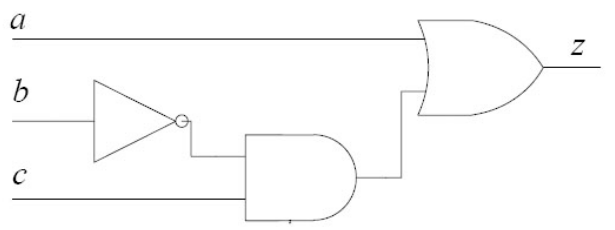
\includegraphics[width=0.7\linewidth]{figs/5}
		\caption{}
		\label{fig:5}
	\end{figure}
	Which one of the following minterm lists represents the circuit given above?
		\hfill{\brak{\text{GATE CS 2020}}}
	\begin{enumerate}
		\begin{multicols}{4}
			\item $z = \sum \brak{0,1,3,7}$
			\item $z = \sum \brak{1,4,5,6,7}$
			\item $z = \sum \brak{2,4,5,6,7}$
			\item $z = \sum \brak{2,3,5}$
		\end{multicols}
	\end{enumerate}
	

	
	\item Consider three registers R1, R2, and R3 that store numbers in IEEE-754 single precision floating point format. Assume that R1 and R2 contain the values \brak{\text{in hexadecimal notation}} 0x42200000 and 0xC1200000, respectively.
	
	If $R3 = \dfrac{R1}{R2}$, what is the value stored in R3?
		\hfill{\brak{\text{GATE CS 2020}}}
	\begin{enumerate}
		\begin{multicols}{4}
			\item 0x40800000
			\item 0xC0800000
			\item 0x83400000
			\item 0xC8500000
		\end{multicols}
	\end{enumerate}

	
	\item A computer system with a word length of $32$ bits has a $16$ MB byte-addressable main memory and a $64$ KB, $4$-way set associative cache memory with a block size of $256$ bytes. Consider the following four physical addresses represented in hexadecimal notation.
	
	$A1 = 0x42C8A4,\;\; A2 = 0x546888,\;\; A3 = 0x6A289C,\;\; A4 = 0x5E4880$
	
	Which one of the following is TRUE?
		\hfill{\brak{\text{GATE CS 2020}}}
	\begin{enumerate}
		\begin{multicols}{4}
			\item A1 and A4 are mapped to different cache sets.
			\item A2 and A3 are mapped to the same cache set.
			\item A3 and A4 are mapped to the same cache set.
			\item A1 and A3 are mapped to the same cache set.
		\end{multicols}
	\end{enumerate}
	

	
	\item Let $G = \brak{V,E}$ be a weighted undirected graph and let $T$ be a Minimum Spanning Tree \brak{\text{MST}} of $G$ maintained using adjacency lists. Suppose a new weighted edge $\brak{u,v} \in V \times V$ is added to $G$. The worst case time complexity of determining if $T$ is still an MST of the resultant graph is
		\hfill{\brak{\text{GATE CS 2020}}}
	\begin{enumerate}
		\begin{multicols}{4}
			\item $\Theta\brak{\abs{E} + \abs{V}}$
			\item $\Theta\brak{\abs{E}\abs{V}}$
			\item $\Theta\brak{\abs{E}\log \abs{V}}$
			\item $\Theta\brak{\abs{V}}$
		\end{multicols}
	\end{enumerate}
	

	
	\item Consider the following languages.
	\begin{align*}
		L_{1} &= \{w x y z \mid w,x,y \in \brak{0+1}^{*}\} \\
		L_{2} &= \{x y \mid x,y \in \brak{a+b}^{*}, \abs{x}=\abs{y}, x \neq y\}
	\end{align*}
	
	Which one of the following is TRUE?
		\hfill{\brak{\text{GATE CS 2020}}}
	\begin{enumerate}
			\item $L_{1}$ is regular and $L_{2}$ is context-free.
			\item $L_{1}$ is context-free but not regular and $L_{2}$ is context-free.
			\item Neither $L_{1}$ nor $L_{2}$ is context-free.
			\item $L_1$	is context-free but $L_2$ is not context-free.
	\end{enumerate}


\item Consider the productions $A \to PQ$ and $A \to XY$. Each of the five non-terminals $A$, $P$, $Q$, $X$ and $Y$ has two attributes: $s$ is a synthesized attribute, and $i$ is an inherited attribute. Consider the following rules.  

Rule 1: $P.i = A.i + 2, Q.i = P.i + A.i, \text{ and } A.s = P.s + Q.s$  

Rule 2: $X.i = A.i + Y.s \text{ and } Y.i = X.s + A.i$  

Which one of the following is TRUE?  

\hfill{\brak{\text{GATE CS 2020}}}

\begin{enumerate}
	\begin{multicols}{2}
		\item Both Rule 1 and Rule 2 are L-attributed.
		\item Only Rule 1 is L-attributed.
		\item Only Rule 2 is L-attributed.
		\item Neither Rule 1 nor Rule 2 is L-attributed.
	\end{multicols}
\end{enumerate}

\item Each of a set of $n$ processes executes the following code using two semaphores \texttt{a} and \texttt{b} initialized to 1 and 0, respectively. Assume that \texttt{count} is a shared variable initialized to 0 and not used in CODE SECTION P.

\begin{framed}
	\begin{verbatim}
		CODE SECTION P
	\end{verbatim}
\end{framed}

\begin{verbatim}
	wait(a); count=count+1;
	if (count==n) signal(b);
	signal(a); wait(b); signal(b);
\end{verbatim}

\begin{framed}
	\begin{verbatim}
		CODE SECTION Q
	\end{verbatim}
\end{framed}
What does the code achieve?
\begin{enumerate}
	\item It ensures that no process executes CODE SECTION Q before every process has finished CODE SECTION P.
	\item It ensures that at most two processes are in CODE SECTION Q at any time.
	\item It ensures that all processes execute CODE SECTION P mutually exclusively.
	\item It ensures that at most $n-1$ processes are in CODE SECTION P at any time.
\end{enumerate}

\item Consider the following five disk access requests of the form \brak{\text{request id, cylinder number}} that are present in the disk scheduler queue at a given time.  

\[
(P,155), (Q,85), (R,110), (S,30), (T,115)
\]  

Assume the head is positioned at cylinder $100$. The scheduler follows Shortest Seek Time First scheduling to service the requests.  

Which one of the following statements is FALSE?  

\hfill{\brak{\text{GATE CS 2020}}}

\begin{enumerate}
	\begin{multicols}{2}
		\item Q is serviced after S, but before T.
		\item The head reverses its direction of movement between servicing of Q and P.
		\item R is serviced before P.
		\item P is serviced before R.
	\end{multicols}
\end{enumerate}

\item Consider a relational table $R$ that is in 3NF, but not in BCNF. Which one of the following statements is TRUE?  

\hfill{\brak{\text{GATE CS 2020}}}

\begin{enumerate}
	\item $R$ has a nontrivial functional dependency $X \to A$, where $X$ is not a superkey and $A$ is a prime attribute.
	\item $R$ has a nontrivial functional dependency $X \to A$, where $X$ is not a superkey and $A$ is a non-prime attribute and $X$ is not a proper subset of any key.
	\item $R$ has a nontrivial functional dependency $X \to A$, where $X$ is not a superkey and $A$ is a non-prime attribute and $X$ is a proper subset of some key.
	\item A cell in $R$ holds a set instead of an atomic value.
\end{enumerate}


\item Consider a schedule of transactions \( T_1 \) and \( T_2 \):
\[
\begin{array}{|c|c|c|c|c|c|c|c|c|c|c|}
	\hline
	T_1 & RA &	&	& RC &  & WD &  & WB & \text{Commit} &    \\
	\hline
	T_2 &  & RB & WB &  & RD &  & WC &  &  & \text{Commit} \\
	\hline
\end{array}
\]
Here, RX stands for ``Read(X)'' and WX stands for ``Write(X)''. Which one of the following schedules is conflict equivalent to the above schedule?
\hfill{\brak{\text{GATE CS 2020}}}
\begin{enumerate}[label=(\Alph*)]
	\item \[
	\begin{array}{|c|c|c|c|c|c|c|c|c|c|c|}
		\hline
		T_1 &  &  &  & RA & RC & WD & WB &  &\text{Commit}& \\
		\hline
		T_2 & RB & WB & RD &  &  &  &  & WC &  & \text{Commit} \\
		\hline
	\end{array}
	\]
	
	\item \[
	\begin{array}{|c|c|c|c|c|c|c|c|c|c|c|}
		\hline
		T_1 & RA & RC & WD & WB &  &  & \text{Commit} \\
		\hline
		T_2 &  &  &  &  & RB & WB & RD & WC &  & \text{Commit} \\
		\hline
	\end{array}
	\]
	
	\item \[
	\begin{array}{|c|c|c|c|c|c|c|c|c|c|c|}
		\hline
		T_1 & RA & RC & WD &  & & & WB &  &  \text{Commit} &   \\
		\hline
		T_2 &  &  &  & RB & WB & RD& & WC &  & \text{Commit} \\
		\hline
	\end{array}
	\]
	
	\item \[
	\begin{array}{|c|c|c|c|c|c|c|c|c|c|c|}
		\hline
		T_1&   &   &  &  & RA & RC & WD & WB & \text{Commit} &   \\
		\hline
		T_2 & RB & WB & RD & WC &  &  &  &  &  & \text{Commit} \\
		\hline
	\end{array}
	\]
\end{enumerate}


\item An organization requires a range of IP addresses to assign one to each of its $1500$ computers. The ISP uses CIDR and serves the requests from the available IP address space $202.61.0.0/17$. The ISP wants to assign an address space using route aggregation. Which of the following address spaces are potential candidates from which the ISP can allot any one to the organization?  

I. 202.61.84.0/21  
II. 202.61.104.0/21  
III. 202.61.64.0/21  
IV. 202.61.144.0/21  

\hfill{\brak{\text{GATE CS 2020}}}

\begin{enumerate}
	\begin{multicols}{2}
		\item I and II only
		\item II and III only
		\item III and IV only
		\item I and IV only
	\end{multicols}
\end{enumerate}

\item Which one of the following predicate formulae is NOT logically valid?  

Note that $W$ is a predicate formula without any free occurrence of $x$.  

\hfill{\brak{\text{GATE CS 2020}}}

\begin{enumerate}
	\begin{multicols}{2}
		\item $\forall x \brak{p(x) \to W} \equiv \forall x \; p(x) \to W$
		\item $\exists x \brak{p(x) \wedge W} \equiv \exists x \; p(x) \wedge W$
		\item $\forall x \brak{p(x) \to W} \equiv \forall x \; p(x) \to W$
		\item $\exists x \brak{p(x) \to W} \equiv \exists x \; p(x) \to W$
	\end{multicols}
\end{enumerate}

\item Let $G = (V, E)$ be a directed, weighted graph with weight function $w \colon E \to \mathbb{R}$. For some function $f \colon V \to \mathbb{R}$, for each edge $(u, v) \in E$, define $w'(u,v)$ as $w(u,v) + f(u) - f(v)$.  

Which one of the options completes the following sentence so that it is TRUE?  

“The shortest paths in $G$ under $w$ are shortest paths under $w'$ too, \_\_\_\_\_\_\_.”  

\hfill{\brak{\text{GATE CS 2020}}}

\begin{enumerate}
	\item for every $f \colon V \to \mathbb{R}$
	\item if and only if $\forall u \in V, f(u)$ is positive
	\item if and only if $\forall u \in V, f(u)$ is negative
	\item if and only if $f(u)$ is the distance from $s$ to $u$ in the graph obtained by adding a new vertex $s$ to $G$ and edges of zero weight from $s$ to every vertex of $G$
\end{enumerate}

\item In a balanced binary search tree with $n$ elements, what is the worst case time complexity of reporting all elements in range $\brak{a, b}$? Assume that the number of reported elements is $k$.  

\hfill{\brak{\text{GATE CS 2020}}}

\begin{enumerate}
	\begin{multicols}{4}
		\item $\Theta(\log n)$
		\item $\Theta(\log n + k)$
		\item $\Theta(\log n + \log k)$
		\item $\Theta(n \log k)$
	\end{multicols}
\end{enumerate}

\item The number of permutations of the characters in LILAC so that no character appears in its original position, if the two L’s are indistinguishable, is \underline{\hspace{2cm}}.  

\hfill{\brak{\text{GATE CS 2020}}}

\item Consider a non-pipelined processor operating at $2.5$ GHz. It takes $5$ clock cycles to complete an instruction. You are going to make a $5$-stage pipeline out of this processor. Overheads associated with pipelining force you to operate the pipelined processor at $2$ GHz. In a given program, assume that $30\%$ are memory instructions, $60\%$ are ALU instructions and the rest are branch instructions. $5\%$ of the memory instructions cause stalls of $50$ clock cycles each due to cache misses and $50\%$ of the branch instructions cause stalls of $2$ cycles each. Assume that there are no stalls associated with the execution of ALU instructions. For this program, the speedup achieved by the pipelined processor over the non-pipelined processor (round off to 2 decimal places) is \underline{\hspace{2cm}}.  

\hfill{\brak{\text{GATE CS 2020}}}

\item A processor has $64$ registers and uses $16$-bit instruction format. It has two types of instructions: I-type and R-type. Each I-type instruction contains an opcode, a register name, and a $4$-bit immediate value. Each R-type instruction contains an opcode and two register names. If there are $8$ distinct I-type opcodes, then the maximum number of distinct R-type opcodes is \underline{\hspace{2cm}}.  

\hfill{\brak{\text{GATE CS 2020}}}

\item For $n > 2$, let $a \in \{0,1\}^n$ be a non-zero vector. Suppose that $x$ is chosen uniformly at random from $\{0,1\}^n$. Then, the probability that $\sum_{i=1}^n a_i x_i$ is an odd number is \underline{\hspace{2cm}}.  

\hfill{\brak{\text{GATE CS 2020}}}

\item Consider the following C functions.
\begin{verbatim}
	int fun1(int n) {
		static int i = 0;
		if (n > 0) {
			++i;
			fun1(n-1);
		}
		return(i);
	}
\end{verbatim}
\begin{verbatim}
	int fun2(int n) {
		static int i = 0;
		if (n > 0) {
			i = i + fun1(n);
			fun2(n-1);
		}
		return(i);
	}
\end{verbatim}
The return value of \texttt{fun2(5)} is \underline{\hspace{2cm}}.\\
\item Consider the array representation of a binary min-heap containing 1023 elements. 
The minimum number of comparisons required to find the maximum in the heap is \underline{\hspace{2cm}}.  
\hfill{\brak{\text{GATE CS 2020}}}
\\
\item Consider the following C functions.
\begin{verbatim}
	int tob(int b, int* arr){
		int i;
		for(i=0; b>0; i++){
			if(b%2) arr[i]=1;
			else arr[i]=0;
			b = b/2;
		}
		return(i);
	}
\end{verbatim}
\underline{\hspace{6cm}}\\
\begin{verbatim}
\underline{\hspace{2cm}}.
	int pp(int a, int b){
		int arr[20];
		int i, tot = 1, ex, len;
		ex = a;
		len = tob(b, arr);
		for(i=0; i<len; i++){
			if(arr[i]==1)
			tot = tot * ex;
			ex = ex * ex;
		}
		return(tot);
	}
\end{verbatim}
The value returned by \texttt{pp(3,4)} is \underline{\hspace{2cm}}.  
\hfill{\brak{\text{GATE CS 2020}}}

\item Consider a graph $G = (V,E)$, where $V = \{v_1,v_2,\dots,v_{100}\}, 
E = \{(v_i,v_j) \mid 1 \leq i < j \leq 100\}$, and weight of the edge $(v_i,v_j)$ is $|i-j|$.  
The weight of the minimum spanning tree of $G$ is \underline{\hspace{2cm}}.  
\hfill{\brak{\text{GATE CS 2020}}}

\item Consider the following set of processes, assumed to have arrived at time 0. 
Consider the CPU scheduling algorithms Shortest Job First (SJF) and Round Robin (RR). 
For RR, assume that the processes are scheduled in the order $P_1,P_2,P_3,P_4$.\\
\begin{center}
	\begin{tabular}{|c|c|c|c|c|}
		\hline
		Processes & $P_1$ & $P_2$ & $P_3$ & $P_4$ \\
		\hline
		Burst time (in ms) & 8 & 7 & 2 & 4 \\
		\hline
	\end{tabular}
\end{center}
If the time quantum for RR is 4 ms, then the absolute value of the difference between the average turnaround times (in ms) of SJF and RR (round off to 2 decimal places) is \underline{\hspace{2cm}}.  \hfill{\brak{\text{GATE CS 2020}}}

\item Consider the following language.
\[
L = \{x \in \{a,b\}^* \mid \text{number of a's in $x$ is divisible by 2 but not divisible by 3}\}
\]

The minimum number of states in a DFA that accepts $L$ is \underline{\hspace{2cm}}.
\hfill{\brak{\text{GATE CS 2020}}}\\
\item Graph $G$ is obtained by adding vertex $s$ to $K_{3,4}$ and making $s$ adjacent to every vertex of $K_{3,4}$.  
The minimum number of colours required to edge-colour $G$ is \underline{\hspace{2cm}}.  
\hfill{\brak{\text{GATE CS 2020}}}\\

\item Consider a paging system that uses 1-level page table residing in main memory and a TLB for address translation. Each main memory access takes $100$ ns and TLB lookup takes $20$ ns. Each page transfer to/from the disk takes $5000$ ns. Assume that the TLB hit ratio is $95\%$, page fault rate is $10\%$. Assume that for $20\%$ of the total page faults, a dirty page has to be written back to disk before the required page is read in from disk. TLB update time is negligible. The average memory access time in ns \brak{\text{round off to 1 decimal places}} is \underline{\hspace{2cm}}.
\hfill{\brak{\text{GATE CS 2020}}}\\
 
\item Consider a database implemented using B+ tree for file indexing and installed on a disk drive with block size of $4$ KB. The size of search key is $12$ bytes and the size of tree/disk pointer is $8$ bytes. Assume that the database has one million records. Also assume that no node of the B+ tree and no records are present initially in main memory. Consider that each record fits into one disk block. The minimum number of disk accesses required to retrieve any record in the database is \underline{\hspace{2cm}}.
\hfill{\brak{\text{GATE CS 2020}}}\\
 
\item Consider a TCP connection between a client and a server with the following specifications: the round trip time is $6$ ms, the size of the receiver advertised window is $50$ KB, slow-start threshold at the client is $32$ KB, and the maximum segment size is $2$ KB. The connection is established at time $t = 0$. Assume that there are no timeouts and errors during transmission. Then the size of the congestion window \brak{\text{in KB}} at time $t + 60$ ms after all acknowledgements are processed is \underline{\hspace{2cm}}.
\hfill{\brak{\text{GATE CS 2020}}}
	

\end{enumerate}
\end{document}
